% Roll Number 30, George Phili Puthiyote

\textbf{\textcolor{LightMagenta}{Calculate output of the following neuron Y if the activation function is . (December 2018 Q6)
\begin{enumerate}
         \item Binary Sigmoid
         \item Bipolar Sigmoid \hfill 4 marks
\end{enumerate}}}
\begin{figure}[htp]
    \centering
    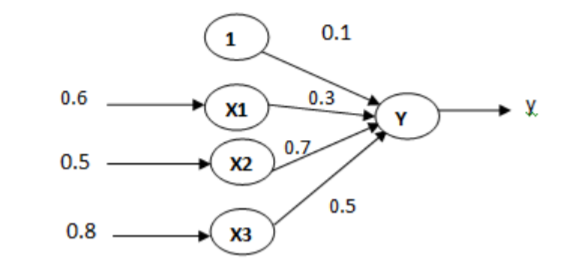
\includegraphics[width=10cm]{Images/A6_img1.png}
\end{figure}

Let input of activation function be x\\
x = 1 x w1 + X1 x w2 + X2 x w3 + X3 x w4\\
x = 1 x 0.1 + 0.6 x 0.3 + 0.5 x 0.7 + 0.8 x 0.5\\
x = 0.1 + 0.18 + 0.35 + 0.40\\
x = 1.03\\
Output of neuron is y


\begin{enumerate}
         \item $$ Binary Sigmoid =  \frac{\mathrm{1} }{\mathrm{1} + e^{-x} } $$
         $$ y = \frac{\mathrm{1} }{\mathrm{1} + e^{-1.03} } = 0.7369$$
         
         
         \item $$Bipolar Sigmoid = -1 + \frac{\mathrm{2} }{\mathrm{1} + e^{-x} } $$\\
         $$ y = -1 + \frac{\mathrm{2} }{\mathrm{1} + e^{-1.03} } = -0.4738 $$\\
 \end{enumerate}